\documentclass[letterpaper, twoside,12pt]{article}
\usepackage{amsmath}
\usepackage{amssymb}
\usepackage{graphics}
\usepackage{float}
\usepackage{tikz}
\usetikzlibrary{arrows.meta, calc, matrix, fit}
\usepackage{nicematrix}
\usepackage{colortbl}

\setlength{\parskip}{1em}

\title{Single Array Square Grid (SASQUARE)}
\date{2021-xx-xx}
\author{Kurt M. Ma. Coll}

\begin{document}
    \pagenumbering{gobble}

    \maketitle
    \newpage
    \pagenumbering{roman}

    \tableofcontents
    \newpage

    \section*{Introduction}
    In computer science, a developer uses an array to represent a series of elements of the same data type such as integers or characters. It is a data structure that holds a list of elements; each of the elements is indexed to determine its position in the list. In mathematics, the best way to represent an array is to create a row vector, a matrix with only one row. We will use a matrix because a set is unordered and does not use indices to ordinally label its elements.

    When representing an n-by-n or a square grid using arrays, a developer will intuitively use two-dimensional arrays to represent the rows and columns. In each array that represents a row, there are arrays that represent different columns. However, we can represent a square grid with only one array that can later be translated into a two-dimensional array.

    This paper aims to illustrate the conversion of a row vector with a perfect square number of elements into a perfect square matrix or vice-versa to represent a square grid.

    \newpage
    \pagenumbering{arabic}
    \setcounter{section}{-1}

    \section{Preliminaries}
    Most of the following equations in this book are heavily reliant on the ceiling and floor functions. According to Iverson (1962), these two functions are used to approximate a number by an integer. We will use his notations for the ceiling function and the floor function.

    \subsection{The Ceiling Function}

    We will denote the application of the ceiling function on a real number like this:
    \begin{equation}
        y = \left\lceil x \right\rceil
    \end{equation}
    Let $x$ be any real number. The value of $y$ will be equal to $x$ only when $x$ is also an integer or a whole number, having no fractional parts or its decimal part is 0. If $x$ is a positive real number, we will remove its fractional part or turn its decimal part into zero, then we will add 1. If $x$ is a negative real number, we will just simply remove the fractional part or turn the decimal part into zero.

    The number 3.14 is a real number and has a decimal part of .14, we will remove the decimal part of 3.14 and add 1 to it.
    \begin{equation*}
        y = \left\lceil 3.14 \right\rceil = 4
    \end{equation*}

    The number $-6\frac{1}{4}$ is a mixed number and has a fractional part of $\frac{1}{4}$, we will remove the fractional part of $-6\frac{1}{4}$ and do nothing else since $-6\frac{1}{4}$ is a negative number.
    \begin{equation*}
        y = \left\lceil -6\frac{1}{4} \right\rceil = -6
    \end{equation*}

    Any improper function must first be solved by dividing the numerator by the denominator. Should there be a remainder, we will increment the quotient by 1, otherwise, we leave the quotient as is.
    \begin{equation*}
        \begin{split}
            y &= \left\lceil \frac{24}{5} \right\rceil \\
            y &= \left\lceil 4\frac{4}{5} \right\rceil \\
            y &= 5
        \end{split}
    \end{equation*}

    The number $\frac{-49}{5}$ is a negative real number. The division must be done first. We will just retain the quotient for it is a negative number; the result will be -9.
    \begin{equation*}
        \begin{split}
            y &= \left\lceil \frac{-49}{5} \right\rceil \\
            y &= \left\lceil -9\frac{4}{5} \right\rceil \\
            y &= -9
        \end{split}
    \end{equation*}

    Whether the number is positive or negative, as long as it is an integer, we will leave it as is.
    \begin{equation*}
        \begin{split}
            y &= \left\lceil 69.0 \right\rceil = 69\\
            y &= \left\lceil -69.0 \right\rceil = -69\\
        \end{split}
    \end{equation*}

    \subsection{The Floor Function}
    The floor function is the opposite of the ceiling function. We will denote it like this:
    \begin{equation}
        y = \left\lfloor x \right\rfloor
    \end{equation}
    Should $x$ be an integer, we will leave it as is. However, should it be a positive real number, we will just turn its decimal part into 0 or remove the fractional part. Should it be a negative real number, not only we will remove the fractional part but we will also subtract 1 from it.

    We simply turned the decimal part into 0 since 3.14 is a positive real number.
    \begin{equation*}
        y = \left\lfloor 3.14 \right\rfloor = 3
    \end{equation*}

    The number $-6\frac{1}{4}$ is a negative mixed number, we removed its fractional part and subtracted 1 from -6.
    \begin{equation*}
        y = \left\lfloor -6\frac{1}{4} \right\rfloor = -7
    \end{equation*}

    Any improper function must first be solved by dividing the numerator by the denominator. Should there be a remainder, it will be just ignored and the whole part will be the result.
    \begin{equation*}
        \begin{split}
            y &= \left\lfloor \frac{24}{5} \right\rfloor \\
            y &= \left\lfloor 4\frac{4}{5} \right\rfloor \\
            y &= 4
        \end{split}
    \end{equation*}

    Should there be a remainder and the mixed number itself is negative, we will subtract 1 from the whole number as a result.
    \begin{equation*}
        \begin{split}
            y &= \left\lfloor \frac{-49}{5} \right\rfloor \\
            y &= \left\lfloor -9\frac{4}{5} \right\rfloor \\
            y &= -10
        \end{split}
    \end{equation*}

    Whether the number is positive or negative, as long as it is an integer, we will leave it as is.
    \begin{equation*}
        \begin{split}
            y &= \left\lfloor 69.0 \right\rfloor = 69\\
            y &= \left\lfloor -69.0 \right\rfloor = -69\\
        \end{split}
    \end{equation*}

    \subsection{Floor and Ceiling of a Zero Whole Part Number}
    The equations $\left\lceil x \right\rceil = 1$ and $\left\lfloor x \right\rfloor = 0$ are true when $0 < x < 1$ and $x$ is a real number.

    The equations $\left\lceil x \right\rceil = 0$ and $\left\lfloor x \right\rfloor = 1$ are true when $-1 < x < 0$ and $x$ is a real number.


    \newpage

    \section{The Square Grid} \label{1_square_grid}
    We will represent a single array with square number of indices using a row vector. The array elements shall be indexed from 1 up to the number of elements.\footnote{Programming languages, such as Python or C, often start their array indices from 0 rather than 1. Since this is a math paper, we will start with 1}
    \begin{figure}[ht]
    \centering
    \resizebox{\textwidth}{!}{%
    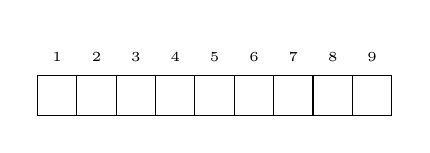
\begin{tikzpicture} [nodes in empty cells,
        nodes={minimum width=0.5cm, minimum height=0.5cm},
        row sep=-\pgflinewidth, column sep=-\pgflinewidth]
    %    border/.style={draw}
    
        \matrix(vector)[matrix of nodes, ampersand replacement=\&, % <- added ampersand replacement
        row 1/.style={nodes={draw=none, minimum width=0.3cm}},
        nodes={draw}]
        { % use \& instead of & as column separator
            \tiny{1} \& \tiny{2} \& \tiny{3} \& \tiny{4} \& \tiny{5} \& \tiny{6} \& \tiny{7} \& \tiny{8} \& \tiny{9}\\
             \& \& \& \& \& \& \& \& \\
        };
        \end{tikzpicture}%
    }
    \caption{A grid representation of a single array} \label{1f1}
    \end{figure}

    \begin{figure}[ht]
        \centering
        \resizebox{\textwidth}{!}{$
        A = 
        \begin{bmatrix}
        a_{1,1} & a_{1,2} & a_{1,3} & a_{1,4} & a_{1,5} & a_{1,6} & a_{1,7} & a_{1,8} & a_{1,9}
        \end{bmatrix}
        $}
        \caption{The array is represented as a row vector} \label{row_vector_form}
    \end{figure}

    Let $i_n$ be an array element of sequence $I$; this is the notation for an ordered list of numbers. Since the row vector has only one row, we will use this indexing notation to represent an element of the row vector. For example, we will represent the 7th element of the array as $i_7$ which is $a_{1,7}$ when indexed as an element of a row vector. The sequence form of the array in Figure \ref{row_vector_form} is:
    \begin{equation}
        A = (i_1,i_2,i_3,i_4,i_5,i_6,i_7,i_8,i_9)
    \end{equation}

    \subsection{The Base of the Square} \label{base}
    The \textbf{base} of a square is the root of the square. We will use it in most of the following expressions to determine particular parts of a square grid. Throughout the paper, we'll represent the base as $b$. 

    Let $b^2$ be any positive non-zero integer. The root of a perfect square can be positive or negative; for the sake of simplicity, we will use positive bases only. The number of elements in a matrix or an array is always an integer.

    \subsection{The Cells} \label{cells}
    The \textbf{}{cells} are the basic building blocks of a grid. Since a square matrix can be thought of as a grid, we will call the elements of an array or a matrix as cells. The number of cells in a square grid counts from 1 up to $b^2$ in either its row vector form or its square matrix form. We shall use integers to index each cell and call each index a cell index.
    \begin{equation}
        (i_n)^{b^2}_{n\in\mathbb{Z}^+} = (i_1, i_2, \dots ,i_{b^2})
    \end{equation}

    A square grid has rows and columns. The total number of rows in a square grid is equals to $b$ which is also equal to the total number of columns in a square grid. We will index $b$ number of rows from 1 to $b$; we will call this each index a row index. We will also do the same to the $b$ number of columns and call each index a column index. The aforementioned indices are all positive integers. Usually an array is expressed as $A_{m \times n}$ or $A_{r \times c}$. In a square matrix, $m = n$ or $r = c$. For convention, we will use $A_{r \times c}$ for expressing a square grid as a square matrix or $A_{b}$ as a row vector.
    \begin{figure}[ht]
        \centering
        \begin{minipage}{0.45\textwidth}
            \centering
            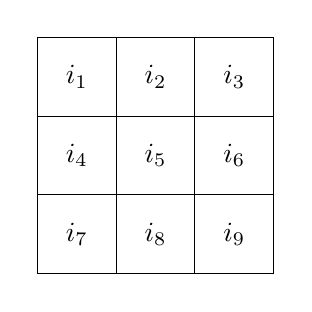
\begin{tikzpicture}
                \matrix[matrix of nodes, nodes={minimum size=1cm, draw, anchor=center}, row sep=-\pgflinewidth, column sep=-\pgflinewidth](mygrid){%
                $i_1$ & $i_2$ & $i_3$ \\
                $i_4$ & $i_5$ & $i_6$ \\
                $i_7$ & $i_8$ & $i_9$ \\
                };
            \end{tikzpicture}
        \end{minipage}
        \begin{minipage}{0.45\textwidth}
            \centering
            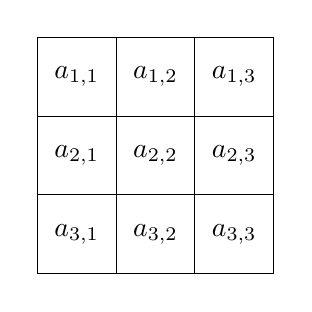
\begin{tikzpicture}
                \matrix[matrix of nodes, nodes={minimum size=1cm, draw, anchor=center}, row sep=-\pgflinewidth, column sep=-\pgflinewidth](mygrid){%
                $a_{1,1}$ & $a_{1,2}$ & $a_{1,3}$ \\
                $a_{2,1}$ & $a_{2,2}$ & $a_{2,3}$ \\
                $a_{3,1}$ & $a_{3,2}$ & $a_{3,3}$ \\
                };
            \end{tikzpicture}
        \end{minipage}

        \caption{Two square grids are labeled differently, they are indexed as elements of a sequence and a matrix respectively} \label{2forms1grid}
    \end{figure}

    In Figure \ref{2forms1grid}, the base of the square grids is 3 and the total number of cells is 9. In matrix notation, the rows and columns are indexed accordingly. We denote the elements of the right grid with $a_{r,c}$ where $r$ is the row index and $c$ is the column index. In this example, we assume that both grids represent the same array.

    \subsection{The Rows} \label{rows}
    The \textbf{rows} are the horizontal arrangement of elements in a matrix. In a row, there are $b$ number of cells. We shall denote a row index as $a_{r,*}$. We shall use function $r$ to determine the row of cell index $n$ in a square grid of base $b$.
    \begin{equation}
        r(b,n) = \left\lceil \frac{n}{b} \right\rceil
    \end{equation}
    We can use the function to determine which multiple of $b$ is \emph{higher} than and nearest to cell $n$ by multiplying its results to $b$. All the rightmost cells of the grid is always indexed with a number divisible by $b$. Let $a_{r,b}$ the rightmost cell index of a row.
    \begin{equation}
        a_{r,b} = b\left\lceil \frac{n}{b} \right\rceil
    \end{equation}

    \subsection{The Columns} \label{columns}
    The \textbf{columns} are the vertical arrangement of elements in a matrix. In a column, there are $b$ number of cells. We shall denote a column index as $a_{*,c}$. To find the column where a cell belongs, we must first identify the row where it belongs and find the rightmost cell of the row. After finding the rightmost cell of the row, we shall subtract it from the sum of the cell index $n$ and the base. We shall use function $c$.
    \begin{equation}
        c(b,n) = n + b - b\left\lceil \frac{n}{b} \right\rceil
    \end{equation}

    All the rightmost cells belong in column index $b$ which is represented as $a_{*,b}$.

    \newpage

    \subsection{Example: Row and Column of Cell 17 in 5-Square}
    \label{1_example_1}
    \begin{figure*}[ht]
        \centering
        \setcounter{MaxMatrixCols}{25}
            \tikzset{highlight/.style={
                rectangle,
                fill=gray!55,
                blend mode = multiply,
                rounded corners = 0.7 mm,
                inner sep=1pt,
                fit = #1}
            }
            \centering
            $I_5 =$
            \resizebox{\textwidth}{!}{$
            \begin{bNiceMatrix}
                i_{1} & i_{2} & i_{3} & i_{4} & i_{5} & i_{6} & i_{7} & i_{8} & i_{9} & i_{10} & i_{11} & i_{12} & i_{13} & i_{14} & i_{15} & i_{16} & i_{17} & i_{18} & i_{19} & i_{20} & i_{21} & i_{22} & i_{23} & i_{24} & i_{25}
                \CodeAfter 
                    \tikz \node [highlight=(1-17)] {};
            \end{bNiceMatrix}
            $}
    \end{figure*}

    The row vector $I$ is a square grid of base 5; to which row does cell $i_{17}$ belong to and what is the rightmost cell in that row? We shall start by using function $r$.
    \begin{equation*}
        \begin{split}
            r(b,n) &= \left\lceil \frac{n}{b} \right\rceil \\
            r(5,17) &= \left\lceil \frac{17}{5} \right\rceil \\
                &= 4
        \end{split}
    \end{equation*}

    Cell 17 belongs to row 4 . We shall substitute 4 to $r$ and 5 to $b$ in $a_{r,b}$.
    \begin{equation*}
        \begin{split}
            a_{r,b} &= b\left\lceil \frac{n}{b} \right\rceil \\
            a_{4,5} &= 5(4) \\
            a_{4,5} &= 20 \\
        \end{split}
    \end{equation*}

    The index of the rightmost cell of row 4 is 20; Cell $i_{17}$ and $i_{20}$ belong together in the same row. Next, we shall determine which column $i_{17}$ belongs to.
    \begin{equation*}
        \begin{split}
            c(b,n) &= n + b - b\left\lceil \frac{n}{b} \right\rceil \\
            c(5,17) &= 17 + 5 - 5\left\lceil \frac{17}{5} \right\rceil \\
                &= 17 + 5 - 5(4) \\
                &= 17 + 5 - 20 \\
                &= 22 - 20 \\
            c(5,17) &= 2
        \end{split}
    \end{equation*}

    \newpage

    If $i_{17}$ belongs to row $a_{4,*}$ and column $a_{*,2}$, then $i_{17} = a_{4,2}$.

    \begin{figure*}[ht]
        \centering
        \begin{minipage}{0.45\textwidth}
            \setcounter{MaxMatrixCols}{5}
                \tikzset{highlight/.style={
                    rectangle,
                    fill=gray!55,
                    blend mode = multiply,
                    rounded corners = 0.7 mm,
                    inner sep=1pt,
                    fit = #1}
                }
                \centering
                \resizebox{\textwidth}{!}{$
                I =
                \begin{bNiceMatrix}
                    i_{1} & i_{2} & i_{3} & i_{4} & i_{5} \\
                    i_{6} & i_{7} & i_{8} & i_{9} & i_{10} \\
                    i_{11} & i_{12} & i_{13} & i_{14} & i_{15} \\
                    i_{16} & i_{17} & i_{18} & i_{19} & i_{20} \\
                    i_{21} & i_{22} & i_{23} & i_{24} & i_{25}
                    \CodeAfter 
                        \tikz \node [highlight=(4-2)] {};
                \end{bNiceMatrix}
                $}
        \end{minipage}
        \hfill
        \begin{minipage}{0.45\textwidth}
            \tikzset{
                highlight/.style={
                    rectangle,
                    fill=gray!55,
                    blend mode = multiply,
                    rounded corners = 0.7 mm,
                    inner sep=1pt,
                    fit = #1
                }
            }
            \centering
            \resizebox{\textwidth}{!}{$
            =
            \begin{bNiceMatrix}
                a_{1,1} & a_{1,2} & a_{1,3} & a_{1,4} & a_{1,5} \\
                a_{2,1} & a_{2,2} & a_{2,3} & a_{2,4} & a_{2,5} \\
                a_{3,1} & a_{3,2} & a_{3,3} & a_{3,4} & a_{3,5} \\
                a_{4,1} & a_{4,2} & a_{4,3} & a_{4,4} & a_{4,5} \\
                a_{5,1} & a_{5,2} & a_{5,3} & a_{5,4} & a_{5,5}
                \CodeAfter 
                    \tikz \node [highlight=(4-2)] {};
            \end{bNiceMatrix}
            $}
        \end{minipage}
    \end{figure*}

    \newpage

    \section{The Intersection} \label{intersection}
    All cells belong to only one row and one column, hence $i_n$ can become $a_{r,c}$. An \textbf{intersection} is where a row and a column meet; they can only meet in one cell. The result of an intersection can be represented as either $i_n$ or $a_{r,c}$. As long as $r=c$ in matrix $A_{r \times c}$, any given pair of row and column index will always have an intersection.

    If we can determine the row and column index of a cell index with a given base, we can also determine the cell index that results of intersection a row and a column. To do so, we'll use the function $i$ which can be expressed in three ways. Let $r$ and $c$ be the row and column index respectively.
    \begin{equation}
        \begin{split}
            i(b,r,c) &= b(r-1) + c \\
                    &= br + (b - c) \\
                    &= br - b + c \\
        \end{split}
    \end{equation}
    In the first expression, the part $b(r-1)$ highlights the first $r$ rows where only $c$ number of cells are only highlighted on the last row. The second expression, highlights the $r$ number of rows then the last $(b - c)$ number of cells will be un-highlighted thereafter. The last one is the simplest form amongst the expressions.

    In the only example of Chapter \ref{1_square_grid} (Section \ref{1_example_1}), we used the functions $r$ and $c$ to determine the matrix notation for $i_{17}$ which is $a_{4,2}$. Cell index 17 belongs to row index 4 and column index 2. We shall use function $i$ to test if the intersection of $a_{4,*}$ and $a_{*,2}$ is $i_{17}$ when the $b$ is 5.
    \begin{equation*}
        \begin{split}
            i(b,r,c) &= br - b + c \\
            i(5,4,2) &= (5)(4) - (5) + (2) \\
                &= 20 - 5 + 2 \\
                &= 15 + 2 \\
            i(5,4,2) &= 17
        \end{split}
    \end{equation*}

    This function can be used to enumerate the cells in a chosen row or column.

    \newpage

    \subsection{Cells of a Row} \label{row_cells}
    To enumerate the cells of a row, we will use the Intersection function $i$. A row shall be considered a set of cell indices. Per Chapter \ref{1_square_grid}, the number of cells in a certain row is always $b$.
    \begin{equation}
        \begin{split}
            i(b,r,c) &= br - b + c \\
            a_{r,*}b &= \{ i(b,r,c) : c \in (1, \dots, b) \}
        \end{split}
    \end{equation}
    The expression $a_{r,*}b$ simply means `Row $r$ of $b$-square'. Numbers $b$ and $r$ are constants inside the set builder notation.

    \subsection{Cells of a Column} \label{column_cells}
    To enumerate the cells of a column, we will use the Intersection function $i$. Just like a row, a column is also a set of cell indices. Just like rows, a column has only $b$ number of cells.
    \begin{equation}
        \begin{split}
            i(b,r,c) &= br - b + c \\
            a_{*,c}b &= \{ i(b,r,c) : r \in (1, \dots, b) \}
        \end{split}
    \end{equation}
    The expression $a_{*,c}b$ simply means `Column $c$ of $b$-square'. Numbers $b$ and $c$ are constants inside the set builder notation.

    \subsection{Example: The Cells of Row 4 and Column 2 in 5-square} \label{2_example_1}
    To enumerate the cell indices of $a_{4,*}5$ we shall use function $i$ in a set builder notation where $r$ and $b$ is constant.
    \begin{equation*}
        \begin{split}
            i(b,r,c) &= br - b + c \\
            a_{r,*}b &= \{ i(b,r,c) : c \in (1, \dots, b) \} \\
            a_{4,*}5 &= \{ i(5,4,c) : c \in (1,2,3,4,5) \} \\
            \\
            i(5,4,1) &= (5)(4) - 5 + 1 = 16 \\
            i(5,4,2) &= (5)(4) - 5 + 2 = 17 \\
            i(5,4,3) &= (5)(4) - 5 + 3 = 18 \\
            i(5,4,4) &= (5)(4) - 5 + 4 = 19 \\
            i(5,4,5) &= (5)(4) - 5 + 5 = 20 \\
            a_{4,*}5 &= \{16, 17, 18, 19, 20 \} \\
        \end{split}
    \end{equation*}

    The set $a_{4,*}5$ has cell indices $i_{16}, i_{17}, i_{18}, i_{19}$, and $i_{20}$.

    To enumerate the cell indices of $a_{*,2}5$ we shall use function $i$ in a set builder notation where $c$ and $b$ is constant.
    \begin{equation*}
        \begin{split}
            i(b,r,c) &= br - b + c \\
            a_{r,*}b &= \{ i(b,r,c) : r \in (1, \dots, b) \} \\
            a_{4,*}5 &= \{ i(5,r,2) : r \in (1,2,3,4,5) \} \\
            \\
            i(5,1,2) &= (5)(1) - 5 + 2 = 2 \\
            i(5,2,2) &= (5)(2) - 5 + 2 = 7 \\
            i(5,3,2) &= (5)(3) - 5 + 2 = 12 \\
            i(5,4,2) &= (5)(4) - 5 + 2 = 17 \\
            i(5,5,2) &= (5)(5) - 5 + 2 = 22 \\
            a_{*,2}5 &= \{2, 7, 12, 17, 22 \} \\
        \end{split}
    \end{equation*}

    The set $a_{*,2}5$ has cell indices $i_{2}, i_{7}, i_{12}, i_{17}$, and $i_{22}$.

    Set $a_{4,*}5$ and set $a_{*,2}5$, will always meet at one cell; all pairs of $a_{r,*}b$ and $a_{*,c}b$ shall always have an intersection.
    \begin{equation*}
        \begin{split}
            a_{4,*}5 &= \{16, 17, 18, 19, 20 \} \\
            a_{*,2}5 &= \{2, 7, 12, 17, 22 \} \\
            a_{4,*}5 \cap a_{*,2}5 &= \{17\}
        \end{split}
    \end{equation*}

    The intersection of $a_{4,*}5$ and $a_{*,2}5$ is $i_{17}$ or $a_{4,2}$.

    \begin{figure*}[ht]
        \centering
        \begin{minipage}{0.45\textwidth}
            \setcounter{MaxMatrixCols}{5}
                \tikzset{row_hl/.style={
                    line width=0.8pt,
                    draw=gray!80,
                    rectangle,
                    fill=gray!55,
                    blend mode = multiply,
                    rounded corners = 0.7 mm,
                    inner sep=1pt,
                    fit = #1}
                }
                \tikzset{col_hl/.style={
                    rectangle,
                    fill=black!45,
                    blend mode = multiply,
                    rounded corners = 0.7 mm,
                    inner sep=1pt,
                    fit = #1}
                }
                \centering
                \resizebox{\textwidth}{!}{$
                I =
                \begin{bNiceMatrix}
                    i_{1} & i_{2} & i_{3} & i_{4} & i_{5} \\
                    i_{6} & i_{7} & i_{8} & i_{9} & i_{10} \\
                    i_{11} & i_{12} & i_{13} & i_{14} & i_{15} \\
                    i_{16} & i_{17} & i_{18} & i_{19} & i_{20} \\
                    i_{21} & i_{22} & i_{23} & i_{24} & i_{25}
                    \CodeAfter 
                        \tikz \node [row_hl=(4-1)(4-5)] {};
                        \tikz \node [col_hl=(1-2)(5-2)] {};
                \end{bNiceMatrix}
                $}
        \end{minipage}
        \hfill
        \begin{minipage}{0.45\textwidth}
            \tikzset{row_hl/.style={
                line width=0.8pt,
                draw=gray!80,
                rectangle,
                fill=gray!55,
                blend mode = multiply,
                rounded corners = 0.7 mm,
                inner sep=1pt,
                fit = #1}
            }
            \tikzset{col_hl/.style={
                rectangle,
                fill=black!45,
                blend mode = multiply,
                rounded corners = 0.7 mm,
                inner sep=1pt,
                fit = #1}
            }
            \centering
            \resizebox{\textwidth}{!}{$
            =
            \begin{bNiceMatrix}
                a_{1,1} & a_{1,2} & a_{1,3} & a_{1,4} & a_{1,5} \\
                a_{2,1} & a_{2,2} & a_{2,3} & a_{2,4} & a_{2,5} \\
                a_{3,1} & a_{3,2} & a_{3,3} & a_{3,4} & a_{3,5} \\
                a_{4,1} & a_{4,2} & a_{4,3} & a_{4,4} & a_{4,5} \\
                a_{5,1} & a_{5,2} & a_{5,3} & a_{5,4} & a_{5,5}
                \CodeAfter 
                \tikz \node [row_hl=(4-1)(4-5)] {};
                \tikz \node [col_hl=(1-2)(5-2)] {};
            \end{bNiceMatrix}
            $}
        \end{minipage}
    \end{figure*}

    \newpage

    \section{The Slants} \label{slants}
    A \textbf{slant} is a special kind of set of cells. We shall define a slant\footnote{We can also use the word `slope', but some readers may confuse it with the mathematical definition of a slope.} with these traits:
    \begin{itemize}
        \item None of the cells in the set belong in the same row
        \item None of the cells in the set belong in the same column
        \item Only one slant has $b$ number of cells; it is the longest slant
        \item Unlike rows and columns, different slants have different number of cells
        \item Two kinds of slants exist, the \textbf{descending} and \textbf{ascending} slants
    \end{itemize}

    In a square grid, there are $2b-1$ number of slants of each kind in a square grid. For example, if the square has a base of 5, there shall be 9 slants for each kind. Let $l$ be a function that takes $b$ as an argument to determine the number of slants in a square.
    \begin{equation}
        \begin{split}
            l(b) &= 2b - 1 \\
            l(5) &= 2(5) - 1 \\
            l(5) &= 9
        \end{split}
    \end{equation}

    \subsection{The Intersection Sum} \label{intersection_sum}
    There are equations that determine the slant a cell belongs to.

    By adding the row and the column index of a cell, we do an \textbf{intersection sum}. If two cells have the same intersection sums, they belong in the same ascending slant. Let $\sigma$ be the intersection sum function and $n$ be the cell index number.
    \begin{equation}
        \begin{split}
            \sigma(b,n) &= r(b,n) + c(b,n) \\
            r(b,n) &= \left\lceil \frac{n}{b} \right\rceil \\
            c(b,n) &= b + n - b\left\lceil \frac{n}{b} \right\rceil \\
            \sigma(b,n) &= ( \left\lceil \frac{n}{b} \right\rceil ) + (b + n - b\left\lceil \frac{n}{b} \right\rceil)\\
            \sigma(b,n) &= \left\lceil \frac{n}{b} \right\rceil + b + n - b\left\lceil \frac{n}{b} \right\rceil\\
        \end{split}
    \end{equation}

    The intersection sum is crucial to finding all the ascending slants in a square grid.
    \begin{figure}[ht]
        \centering
        {$
        \begin{bNiceMatrix}
            2 & 3 & 4 & 5 & 6 \\
            3 & 4 & 5 & 6 & 7 \\
            4 & 5 & 6 & 7 & 8 \\
            5 & 6 & 7 & 8 & 9 \\
            6 & 7 & 8 & 9 & 10
        \end{bNiceMatrix}
        $}
        \caption{This matrix has elements where $i_{n}b$ = $\sigma(b,n)$. $i_{n}b$ means cell index $n$ of $b$-square.}
    \end{figure}

    \subsection{The Intersection Difference} \label{intersection_diff}
    To do an \textbf{intersection difference}, we shall subtract the row index of a cell from the column index of the same cell. If two cells have the same intersection difference, they belong in the same descending slant. Let $\delta$ be the intersection difference function and $n$ be the cell index number.
    \begin{equation}
        \begin{split}
            \delta(b,n) &= c(b,n) - r(b,n)\\
            r(b,n) &= \left\lceil \frac{n}{b} \right\rceil \\
            c(b,n) &= b + n - b\left\lceil \frac{n}{b} \right\rceil \\
            \delta(b,n) &= (b + n - b\left\lceil \frac{n}{b} \right\rceil) - (\left\lceil \frac{n}{b} \right\rceil)\\
            \delta(b,n) &= b + n - b\left\lceil \frac{n}{b} \right\rceil - \left\lceil \frac{n}{b} \right\rceil\\
        \end{split}
    \end{equation}

    A \textbf{reverse intersection difference} occurs when we subtract the column index of a cell from the row index of the same cell. Let $\alpha$ be the reverse intersection difference.
    \begin{equation}
        \begin{split}
            \alpha(b,n) &= r(b,n) - c(b,n)\\
            r(b,n) &= \left\lceil \frac{n}{b} \right\rceil \\
            c(b,n) &= b + n - b\left\lceil \frac{n}{b} \right\rceil \\
            \alpha(b,n) &= \left\lceil \frac{n}{b} \right\rceil - (b + n - b\left\lceil \frac{n}{b} \right\rceil)\\
            \alpha(b,n) &= \left\lceil \frac{n}{b} \right\rceil - b - n + b\left\lceil \frac{n}{b} \right\rceil
        \end{split}
    \end{equation}

    A reverse intersection difference is a negated version of an intersection difference.
    \begin{equation}
        \begin{split}
            \alpha(b,n) &= -(\delta(b,n))\\
            \left\lceil \frac{n}{b} \right\rceil - (b + n - b\left\lceil \frac{n}{b} \right\rceil) &= - ( b + n - b\left\lceil \frac{n}{b} \right\rceil - \left\lceil \frac{n}{b} \right\rceil)\\
            \left\lceil \frac{n}{b} \right\rceil - b - n + b\left\lceil \frac{n}{b} \right\rceil &= - b - n + b\left\lceil \frac{n}{b} \right\rceil + \left\lceil \frac{n}{b} \right\rceil\\
        \end{split}
    \end{equation}
    If we rearrange the terms of the right expression:
    \begin{equation*}
        \left\lceil \frac{n}{b} \right\rceil - b - n + b\left\lceil \frac{n}{b} \right\rceil = \left\lceil \frac{n}{b} \right\rceil - b - n + b\left\lceil \frac{n}{b} \right\rceil
    \end{equation*}

    The intersection difference is crucial to finding all the descending slants in a square grid.

    \begin{figure}[ht]
        \centering
        \begin{minipage}{0.45\textwidth}
            \centering
            {$
            A =
            \begin{bNiceMatrix}
                0 & 1 & 2 & 3 & 4 \\
                -1 & 0 & 1 & 2 & 3 \\
                -2 & -1 & 0 & 1 & 2 \\
                -3 & -2 & -1 & 0 & 1 \\
                -4 & -3 & -2 & -1 & 0
            \end{bNiceMatrix}
            $}
        \end{minipage}
        \hfill
        \begin{minipage}{0.45\textwidth}
            \centering
            {$
            B =
            \begin{bNiceMatrix}
                0 & -1 & -2 & -3 & -4 \\
                1 & 0 & -1 & -2 & -3 \\
                2 & 1 & 0 & -1 & -2 \\
                3 & 2 & 1 & 0 & -1 \\
                4 & 3 & 2 & 1 & 0
            \end{bNiceMatrix}
            $}
        \end{minipage}
        \caption{Matrix $A$ has elements where $i_{n}b = \delta(b,n)$ whilst matrix B has elements where $i_{n}b = \alpha(b,n)$.}
    \end{figure}

    \newpage

    \subsection{The Diagonal} \label{diagonal}
    A matrix has a special set of elements called a \textbf{diagonal}; it is also called the \textbf{main diagonal}. A diagonal consists of elements where $r = c$. In a square grid, a diagonal is the longest descending slant. Its two end cells are always $a_{1,1}$ and $a_{b,b}$.
    \begin{figure}[ht]
        \tikzset{highlight/.style={
            line width=0.8pt,
            draw=gray!80,
            rectangle,
            fill=gray!55,
            blend mode = multiply,
            rounded corners = 0.7 mm,
            inner sep=1pt,
            fit = #1}
        }
        \centering
        {$
        A =
        \begin{bNiceMatrix}
            a_{1,1} & a_{1,2} & a_{1,3} & a_{1,4} & a_{1,5} \\
            a_{2,1} & a_{2,2} & a_{2,3} & a_{2,4} & a_{2,5} \\
            a_{3,1} & a_{3,2} & a_{3,3} & a_{3,4} & a_{3,5} \\
            a_{4,1} & a_{4,2} & a_{4,3} & a_{4,4} & a_{4,5} \\
            a_{5,1} & a_{5,2} & a_{5,3} & a_{5,4} & a_{5,5}
            \CodeAfter 
            \tikz \node [highlight=(1-1)] {};
            \tikz \node [highlight=(2-2)] {};
            \tikz \node [highlight=(3-3)] {};
            \tikz \node [highlight=(4-4)] {};
            \tikz \node [highlight=(5-5)] {};
        \end{bNiceMatrix}
        $}
        \caption{A diagonal is highlighted in a 5-square matrix} \label{fig:diagonal}
    \end{figure}

    To enumerate the cell indices within the diagonal, we shall use the intersection function $i$ (see Chapter \ref{intersection}) where $r = c$. We shall name the set $D$. For this example, $b = 5$ and $n$ is the nth cell of the diagonal. 
    \begin{equation}
        \begin{split}
            i(b,r,c) &= br - b + c \\
            D &= \{ i(b,n,n) : n \in (1, \dots, b) \} \\
            \\
            i(5,1,1) &= (5)(1) - 5 + 1 = 1 \\
            i(5,2,2) &= (5)(2) - 5 + 2 = 7 \\
            i(5,3,3) &= (5)(3) - 5 + 3 = 13 \\
            i(5,4,4) &= (5)(4) - 5 + 4 = 19 \\
            i(5,5,5) &= (5)(5) - 5 + 5 = 25 \\
            D &= \{1, 7, 13, 19, 25 \} \\
        \end{split}
    \end{equation}

    \newpage

    \subsection{The Anti-diagonal} \label{antidiagonal}
    An \textbf{anti-diagonal} is the opposite of the diagonal. An anti-diagonal has cells where $r = b - c + 1$ where $b$ is the base, where $b = r + c$. The intersection sum of all its cells is always $b + 1$. It is the longest ascending slant. Its two end cells are always $a_{b,1}$ and $a_{1,b}$

    \begin{figure}[ht]
        \tikzset{highlight/.style={
            line width=0.8pt,
            draw=gray!80,
            rectangle,
            fill=gray!55,
            blend mode = multiply,
            rounded corners = 0.7 mm,
            inner sep=1pt,
            fit = #1}
        }
        \centering
        {$
        A =
        \begin{bNiceMatrix}
            a_{1,1} & a_{1,2} & a_{1,3} & a_{1,4} & a_{1,5} \\
            a_{2,1} & a_{2,2} & a_{2,3} & a_{2,4} & a_{2,5} \\
            a_{3,1} & a_{3,2} & a_{3,3} & a_{3,4} & a_{3,5} \\
            a_{4,1} & a_{4,2} & a_{4,3} & a_{4,4} & a_{4,5} \\
            a_{5,1} & a_{5,2} & a_{5,3} & a_{5,4} & a_{5,5}
            \CodeAfter 
            \tikz \node [highlight=(5-1)] {};
            \tikz \node [highlight=(4-2)] {};
            \tikz \node [highlight=(3-3)] {};
            \tikz \node [highlight=(2-4)] {};
            \tikz \node [highlight=(1-5)] {};
        \end{bNiceMatrix}
        $}
        \caption{An anti-diagonal is highlighted in a 5-square matrix} \label{fig:antidiagonal}
    \end{figure}

    To enumerate the cell indices within the anti-diagonal, we shall use the function $\Upsilon$ for finding the nth cell of the anti-diagonal. For this example, $b = 5$.
    \begin{equation}
        \begin{split}
            \Upsilon(b,n) &= b^2 - bn + n \\
            A &= \{ \Upsilon(b,n) : n \in (1, \dots, b) \} \\
            \\
            \Upsilon(5,1) &= 5^2 - (5)(1) + (1) = 21\\
            \Upsilon(5,2) &= 5^2 - (5)(2) + (2) = 17\\
            \Upsilon(5,3) &= 5^2 - (5)(3) + (3) = 13\\
            \Upsilon(5,4) &= 5^2 - (5)(4) + (4) = 9\\
            \Upsilon(5,5) &= 5^2 - (5)(5) + (5) = 5\\
            A &= \{ 21, 17, 13, 9, 5 \} \\
        \end{split}
    \end{equation}


    \subsection{The Off-diagonal Cells} \label{offdiagonal_cells}
    The \textbf{off-diagonal cells} are the cells not found in the main diagonal. There are two kinds of off-diagonal cells: the \textbf{superdiagonal} and the \textbf{subdiagonal} cells. The superdiagonal cells are above and right of the main diagonal whilst the subdiagonal cells are below and left the main diagonal.

    Superdiagonal cells has their row index lower than their column index whilst subdiagonal cells have their row index greater than their column index. Using the intersection difference function (see Section \ref{intersection_diff}), we can determine if a cell belongs to the main diagonal, is a superdiagonal cell, or is a subdiagonal cell. Given that $n$ is a cell index:
    \begin{itemize}
        \item If $\delta(b,n) < 0$, it is a subdiagonal cell.
        \item If $\delta(b,n) > 0$, it is a superdiagonal cell.
        \item If $\delta(b,n) = 0$, it belongs to the main diagonal.
    \end{itemize}

    To further illustrate the superdiagonal and subdiagonal cells, we will show two matrices where the highlighted cells together resembles two triangles.

    \begin{figure}[ht]
        \centering
        \begin{minipage}{0.45\textwidth}
            \tikzset{row_hl/.style={
            line width=0.8pt,
            draw=gray!80,
            rectangle,
            fill=gray!55,
            blend mode = multiply,
            inner sep=1pt,
            fit = #1}
            }
            \tikzset{col_hl/.style={
                rectangle,
                fill=black!45,
                blend mode = multiply,
                inner sep=1pt,
                fit = #1}
            }
            \centering
            {$
            \begin{bNiceMatrix}
                i_{1} & i_{2} & i_{3} & i_{4} & i_{5} \\
                i_{6} & i_{7} & i_{8} & i_{9} & i_{10} \\
                i_{11} & i_{12} & i_{13} & i_{14} & i_{15} \\
                i_{16} & i_{17} & i_{18} & i_{19} & i_{20} \\
                i_{21} & i_{22} & i_{23} & i_{24} & i_{25}
                \CodeAfter 
                \tikz \node [row_hl=(1-2)(1-5)] {};
                \tikz \node [row_hl=(2-3)(2-5)] {};
                \tikz \node [row_hl=(3-4)(3-5)] {};
                \tikz \node [row_hl=(4-5)] {};
                \tikz \node [col_hl=(2-1)] {};
                \tikz \node [col_hl=(3-1)(3-2)] {};
                \tikz \node [col_hl=(4-1)(4-3)] {};
                \tikz \node [col_hl=(5-1)(5-4)] {};
            \end{bNiceMatrix}
            $}
        \end{minipage}
        \hfill
        \begin{minipage}{0.45\textwidth}
            \tikzset{row_hl/.style={
            line width=0.8pt,
            draw=gray!80,
            rectangle,
            fill=gray!55,
            blend mode = multiply,
            inner sep=1pt,
            fit = #1}
            }
            \tikzset{col_hl/.style={
                rectangle,
                fill=black!45,
                blend mode = multiply,
                inner sep=1pt,
                fit = #1}
            }
            \centering
            {$
            \begin{bNiceMatrix}
                0 & 1 & 2 & 3 & 4 \\
                -1 & 0 & 1 & 2 & 3 \\
                -2 & -1 & 0 & 1 & 2 \\
                -3 & -2 & -1 & 0 & 1 \\
                -4 & -3 & -2 & -1 & 0
                \CodeAfter 
                \tikz \node [row_hl=(1-2)(1-5)] {};
                \tikz \node [row_hl=(2-3)(2-5)] {};
                \tikz \node [row_hl=(3-4)(3-5)] {};
                \tikz \node [row_hl=(4-5)] {};
                \tikz \node [col_hl=(2-1)] {};
                \tikz \node [col_hl=(3-1)(3-2)] {};
                \tikz \node [col_hl=(4-1)(4-3)] {};
                \tikz \node [col_hl=(5-1)(5-4)] {};
            \end{bNiceMatrix}
            $}
        \end{minipage}
        \caption{The highlighted off-diagonal cells in two matrices.} \label{fig:offdiagonal_cells}
    \end{figure}

    In Figure \ref{fig:offdiagonal_cells}, the cells highlighted with a light shade of gray are the superdiagonal cells. The rest of the highlighted cells are the subdiagonal cells. The unhighlighted cells are the diagonal cells. The left matrix has elements where $i_{n}b = \delta(b,n)$ where $n$ is the cell index and $b$ is the base of the square.

    \subsection{The Anti-offdiagonal Cells}
    The \textbf{anti-offdiagonal cells} are the cells not found in the anti-diagonal. Like the off-diagonal cells, there are two kinds of anti-offdiagonal cells: the \textbf{anti-superdiagonal} and the \textbf{anti-subdiagonal} cells. The anti-superdiagonal cells are above and left of the anti-diagonal whilst the anti-subdiagonal cells are below and right of the anti-diagonal.

    \newpage

    Using the intersection sum (see Section \ref{intersection_sum}) of a cell index, we can determine whether a cell belongs to the anti-diagonal, is an anti-superdiagonal cell, or is an anti-subdiagonal cell. Given that $n$ is a cell index:
    \begin{itemize}
        \item If $\alpha(b,n) < (b + 1)$, it is an anti-superdiagonal cell.
        \item If $\alpha(b,n) > (b + 1)$, it is an anti-subdiagonal cell.
        \item If $\alpha(b,n) = (b + 1)$, it belongs to the anti-diagonal.
    \end{itemize}

    Like the off-diagonal cells, they can resemble triangles.

    \begin{figure}[ht]
        \centering
        \begin{minipage}{0.45\textwidth}
            \tikzset{row_hl/.style={
            line width=0.8pt,
            draw=gray!80,
            rectangle,
            fill=gray!55,
            blend mode = multiply,
            inner sep=1pt,
            fit = #1}
            }
            \tikzset{col_hl/.style={
                rectangle,
                fill=black!45,
                blend mode = multiply,
                inner sep=1pt,
                fit = #1}
            }
            \centering
            {$
            \begin{bNiceMatrix}
                i_{1} & i_{2} & i_{3} & i_{4} & i_{5} \\
                i_{6} & i_{7} & i_{8} & i_{9} & i_{10} \\
                i_{11} & i_{12} & i_{13} & i_{14} & i_{15} \\
                i_{16} & i_{17} & i_{18} & i_{19} & i_{20} \\
                i_{21} & i_{22} & i_{23} & i_{24} & i_{25}
                \CodeAfter 
                \tikz \node [row_hl=(1-1)(1-4)] {};
                \tikz \node [row_hl=(2-1)(2-3)] {};
                \tikz \node [row_hl=(3-1)(3-2)] {};
                \tikz \node [row_hl=(4-1)] {};
                \tikz \node [col_hl=(2-5)] {};
                \tikz \node [col_hl=(3-4)(3-5)] {};
                \tikz \node [col_hl=(4-3)(4-5)] {};
                \tikz \node [col_hl=(5-2)(5-5)] {};
            \end{bNiceMatrix}
            $}
        \end{minipage}
        \hfill
        \begin{minipage}{0.45\textwidth}
            \tikzset{row_hl/.style={
            line width=0.8pt,
            draw=gray!80,
            rectangle,
            fill=gray!55,
            blend mode = multiply,
            inner sep=1pt,
            fit = #1}
            }
            \tikzset{col_hl/.style={
                rectangle,
                fill=black!45,
                blend mode = multiply,
                inner sep=1pt,
                fit = #1}
            }
            \centering
            {$
            \begin{bNiceMatrix}
                2 & 3 & 4 & 5 & 6 \\
                3 & 4 & 5 & 6 & 7 \\
                4 & 5 & 6 & 7 & 8 \\
                5 & 6 & 7 & 8 & 9 \\
                6 & 7 & 8 & 9 & 10
                \CodeAfter 
                \tikz \node [row_hl=(1-1)(1-4)] {};
                \tikz \node [row_hl=(2-1)(2-3)] {};
                \tikz \node [row_hl=(3-1)(3-2)] {};
                \tikz \node [row_hl=(4-1)] {};
                \tikz \node [col_hl=(2-5)] {};
                \tikz \node [col_hl=(3-4)(3-5)] {};
                \tikz \node [col_hl=(4-3)(4-5)] {};
                \tikz \node [col_hl=(5-2)(5-5)] {};
            \end{bNiceMatrix}
            $}
        \end{minipage}
        \caption{The highlighted anti-offdiagonal cells in two matrices.} \label{fig:antioffdiagonal_cells}
    \end{figure}

    In Figure \ref{fig:antioffdiagonal_cells}, the cells highlighted with a light shade of gray are the anti-superdiagonal cells. The rest of the highlighted cells are the anti-subdiagonal cells. The unhighlighted cells are the anti-diagonal cells. The left matrix has elements where $i_{n}b = \alpha(b,n)$ where $n$ is the cell index and $b$ is the base of the square.

    \newpage

    \section{The Slant Indices} \label{slant_indices}
    To index each individual slants in a square grid, we shall use the intersection sum and intersection difference of each cells.

    We shall call the index of a descending slant a \textbf{descending index} or $\kappa$ (kappa) index. To determine the $\kappa$ index of the cell, we shall use function $\kappa$.
    \begin{equation}
        \kappa(b,n) = b + \delta(b,n)
    \end{equation}

    We shall call the index of an ascending slant an \textbf{ascending index} or $\upsilon$ (upsilon) index. To determine the $\upsilon$ index of the cell, we shall use function $\upsilon$.
    \begin{equation}
        \upsilon(b,n) = \alpha(b,n) - 1
    \end{equation}

    To further illustrate the indexed slants, we substituted the values of the matrix elements into their respective descending and ascending indices.

    \begin{figure}[ht]
        \centering
        \begin{minipage}{0.45\textwidth}
            \centering
            {$
            A =
            \begin{bNiceMatrix}
                5 & 6 & 7 & 8 & 9 \\
                4 & 5 & 6 & 7 & 8 \\
                3 & 4 & 5 & 6 & 7 \\
                2 & 3 & 4 & 5 & 6 \\
                1 & 2 & 3 & 4 & 5
            \end{bNiceMatrix}
            $}
        \end{minipage}
        \hfill
        \begin{minipage}{0.45\textwidth}
            \centering
            {$
            B =
            \begin{bNiceMatrix}
                1 & 2 & 3 & 4 & 5 \\
                2 & 3 & 4 & 5 & 6 \\
                3 & 4 & 5 & 6 & 7 \\
                4 & 5 & 6 & 7 & 8 \\
                5 & 6 & 7 & 8 & 9
            \end{bNiceMatrix}
            $}
        \end{minipage}
        \caption{Matrix $A$ has elements equal to their descending index whilst matrix B has elements equal to their ascending index.}
    \end{figure}

    \subsection{The Cardinality of a Given Slant} \label{slant_cardinality}
    Not all slants have the same number of cells. Only $b-1$ pairs of slants of have the same number of cells for each kind of slants. To get the number of cells in a given slant index. Let $x$ be either a descending ($\kappa$) or an ascending ($\upsilon$) index. Let $X$ be a set of cells belonging to a chosen slant. To resolve the ambuiguity that shall arise when we use the vertical bar notation, we shall use $n(X)$ to denote the \textbf{cardinality} of set $X$. We shall use the vertical bars for denoting absolute values.
    \begin{equation}
        n(X) = b - |b - x|
    \end{equation}
    Only slants with index $b$ have the most number of cells which has a count of $b$.

    \subsection{Multiples of the Base Until Its Square} \label{u_and_w}
    Function $f$ shall denote any function in this subsection. Set $X$ shall denote any set in this subsection.
    \begin{equation}\
            X = \{ f(b,x) : x \in \mathbb{N}, 0 \leq x \leq 2b \}
    \end{equation}
    The range of the any set in this subsection has these traits:
    \begin{itemize}
        \item When $x = b$ then $f(b,x) = 0$
        \item When $x = 0$ then $f(b,x) = b^2$
        \item When $0 \leq x \leq b$ then $f(b,x) = b^2 - bx$
    \end{itemize}
    Function $u$ is a function that either yields a multiple of $b$ or subtracts $b$ from $x$ depending on whether $x$ exceeds or fall short of $b$.
    \begin{equation}
        u(b,x) = b^{2 + \left\lfloor -\frac{x}{b} \right\rfloor }|b-x|
    \end{equation}
    \begin{equation}
        U = \{ u(b,x) : x \in \mathbb{N}, 0 \leq x \leq 2b \}
    \end{equation}
    The range of set $U$ has these own traits:
    \begin{itemize}
        \item When $x = 2b$ then $u(b,x) = b$
        \item When $b \leq x \leq 2b$ then $u(b,x) = x - b$
    \end{itemize}

    Function $w$ is a function that either yields a multiple of $b$ or subtracts $x$ from $b$ depending on whether $x$ exceeds or fall short of $b$.
    \begin{equation}
        w(b,x) = |b-x|(b-1) + b^{\left\lfloor \frac{x}{b} \right\rfloor}(b-x)
    \end{equation}
    \begin{equation}
        W = \{ w(b,x) : x \in \mathbb{N}, 0 \leq x \leq 2b \}
    \end{equation}
    The range of set $W$ has these own traits:
    \begin{itemize}
        \item When $x = 2b$ then $w(b,x) = -b$
        \item When $b \leq x \leq 2b$ then $w(b,x) = b - x$
    \end{itemize}

    \subsection{The Cells of a Slant} \label{cells_of_a_slant}
    We will use several notations to describe the different kind of slants and their cells.
    \begin{itemize}
        \item A descending slant is denoted as $\kappa_{x,*}b$ where $x$ is the index of the descending slant. This cansee Section be also called as ``descending slant x"
        \item A cell in a descending slant is denoted as $\kappa_{x,o}b$ where $o$ is the nth cell of descending slant x.
        \item To depict the nth cells of each descending slants we will denote it as $\kappa_{*,o}b$. (eg. All the 1st cells of each descending slant in 5-square is denoted as $\kappa_{*,1}5$.)
        \item An ascending slant is denoted as $\upsilon_{x,*}b$ where $x$ is the index of the ascending slant. This can be also called as ``ascending slant x"
        \item A cell in an ascending slant is denoted as $\upsilon_{x,o}b$ where $n$ is the nth cell of ascending slant x.
        \item To depict the nth cells of each ascending slants we will denote it as $\upsilon_{*,o}b$. (eg. All the 1st cells of each ascending slant in 5-square is denoted as $\upsilon_{*,1}5$.)
    \end{itemize}

    Before enumerating all the cells of a chosen slant, we must first find the cardinality of the chosen slant (see Section \ref{slant_cardinality}). The variable $s$ represents either a descending slant $\kappa$ or an ascending slant $\upsilon$
    \begin{equation}
        n(s_{x,*}b) = b - |b-x|
    \end{equation}


    To enumerate the cells of a descending slant, we shall add the results of the intersection function (see Section \ref{intersection} and \ref{diagonal}) and function $u$ from section \ref{u_and_w}.
    \begin{equation}
        \begin{split}
            \kappa_{x,o}b &= i(b,o,o) + u(b,x) \\
                &= (bo + b + o) + (b^{2 + \left\lfloor -\frac{x}{b} \right\rfloor }|b-x|)
        \end{split}
    \end{equation}

    We shall use the set builder notation to enumerate the cells. Variables $b$ and $x$ will be constant in this equation.
    \begin{equation}
        K = \{ \kappa_{x,o}b : 1 \leq o \leq n(\kappa_{x,*}b) \}
    \end{equation}

    To enumerate the cells of an ascending slant, we shall subtract the results of function $w$ (see Section \ref{u_and_w}) from the results of the function $\Upsilon$ that enumerates the anti-diagonal cells (see Section \ref{antidiagonal}).
    \begin{equation}
        \begin{split}
            \upsilon_{x,o}b &= \Upsilon(b,o) + w(b,x) \\
                &= (b^2 - bo + o) + (|b-x|(b-1)+ b^{\left\lfloor \frac{x}{b} \right\rfloor}(b-x))
        \end{split}
    \end{equation}

    We shall use the set builder notation to enumerate the cells. Variables $b$ and $x$ will be constant in this equation.
    \begin{equation}
        L = \{ \upsilon_{x,o}b : 1 \leq o \leq n(\upsilon_{x,*}b) \}
    \end{equation}

    \subsection{Example: The Descending Slant of Cell 17 in 5-Square} \label{3-4_example_1}
    To find the descending index of $i_{17}$, we shall first find its intersection difference.
    \begin{equation*}
        \begin{split}
            \delta(b,n) &= b + n - b\left\lceil \frac{n}{b} \right\rceil - \left\lceil \frac{n}{b} \right\rceil\\
            \delta(5,17) &= 5 + 17 - 5\left\lceil \frac{17}{5} \right\rceil - \left\lceil \frac{17}{5} \right\rceil\\
                &= 5 + 17 - 5(4) - (4)\\
                &= 5 + 17 - 20 - 4\\
                &= 2 - 4\\
            \delta(5,17) &= -2\\
        \end{split}
    \end{equation*}

    After finding $\delta(5,17)$ we will find the descending index of $i_{17}$.
    \begin{equation*}
        \begin{split}
            \kappa(b,n) &= b - \delta(b,n)\\
            \kappa(5,17) &= 5 + \delta(5,17)\\
                &= 5 + (-2)\\
                &= 5 - 2\\
            \kappa(5,17) &= 3\\
        \end{split}
    \end{equation*}

    The descending index of $i_{17}$ is 3. To find the neighboring cells of $i_{17}$ in descending slant 3, we will find the cardinality of descending slant 3. We will represent any descending slant as a set using the slant notation $\kappa_{x,*}b$. Let $x$ be equal to 3.
    \begin{equation*}
        \begin{split}
            n(\kappa_{x,*}b) &= b - |b - x| \\
            n(\kappa_{3,*}5) &= 5 - |5 - 3| \\
                &= 5 - |2| \\
                &= 5 - 2 \\
            n(\kappa_{3,*}5) &= 3 
        \end{split}
    \end{equation*}
    There are 3 cells in descending slant 3. To list the indices of each cell, we will use a set builder notation.
    \begin{equation*}
        \begin{split}
            \kappa_{3,*}5 &= \{ \kappa_{x,o}b : 1 \leq o \leq n(\kappa_{x,*}b) \} \\
            \kappa_{3,*}5 &= \{ \kappa_{3,o}5 : 1 \leq o \leq 3 \} \\
        \end{split}
    \end{equation*}
    Since there are only 3 cells in the slant, we will enumerate up to the 3rd cell of descending slant 3.
    \begin{equation*}
        \begin{split}
            \kappa_{x,o}b &= (bo + b + o) + (b^{2 + \left\lfloor -\frac{x}{b} \right\rfloor }|b-x|) \\
            \kappa_{3,1}5 &= (5(1) + 5 + 1) + (5^{2 + \left\lfloor -\frac{3}{5} \right\rfloor }|5-3|) = 11\\
            \kappa_{3,2}5 &= (5(2) + 5 + 2) + (5^{2 + \left\lfloor -\frac{3}{5} \right\rfloor }|5-3|) = 17\\
            \kappa_{3,3}5 &= (5(3) + 5 + 3) + (5^{2 + \left\lfloor -\frac{3}{5} \right\rfloor }|5-3|) = 23\\
            \kappa_{3,*}5 &= \{11, 17, 15\}
        \end{split}
    \end{equation*}
    Cell 17 is the 2nd cell of descending slant 3 because $\kappa_{3,2}5 = 17$
    \begin{figure*}[ht]
        \tikzset{highlight/.style={
            line width=0.8pt,
            draw=gray!80,
            rectangle,
            fill=gray!55,
            blend mode = multiply,
            rounded corners = 0.7 mm,
            inner sep=1pt,
            fit = #1}
        }
        \centering
        {$
        \begin{bNiceMatrix}
            i_{1} & i_{2} & i_{3} & i_{4} & i_{5} \\
            i_{6} & i_{7} & i_{8} & i_{9} & i_{10} \\
            i_{11} & i_{12} & i_{13} & i_{14} & i_{15} \\
            i_{16} & i_{17} & i_{18} & i_{19} & i_{20} \\
            i_{21} & i_{22} & i_{23} & i_{24} & i_{25}
            \CodeAfter 
            \tikz \node [highlight=(3-1)] {};
            \tikz \node [highlight=(4-2)] {};
            \tikz \node [highlight=(5-3)] {};
        \end{bNiceMatrix}
        $}
    \end{figure*}

    \subsection{Example: The Ascending Slant of Cell 17 in 5-Square} \label{3-4_example_2}
    To find the ascending index of $i_{17}$, we shall first find its intersection sum.
    \begin{equation*}
        \begin{split}
            \sigma(b,n) &= \left\lceil \frac{n}{b} \right\rceil + b + n - b\left\lceil \frac{n}{b} \right\rceil\\
            \sigma(5,17) &= \left\lceil \frac{17}{5} \right\rceil + 5 + 17 - 5\left\lceil \frac{17}{5} \right\rceil\\
                &= 4 + 5 + 17 - 5(4)\\
                &= 4 + 5 + 17 - 20\\
                &= 4 + 2\\
            \sigma(5,17) &= 6\\
        \end{split}
    \end{equation*}

    The intersection sum of $i_{17}$ is 6. We will find the ascending index of $i_{17}$.
    \begin{equation*}
        \begin{split}
            \upsilon(b,n) &= \sigma(b,n) - 1\\
            \upsilon(5,17) &= \sigma(5,17) - 1\\
                &= 6 - 1\\
            \upsilon(5,17) &= 5\\
        \end{split}
    \end{equation*}

    The ascending index of $i_{17}$ is 5. To find the neighboring cells of $i_{17}$ in ascending slant 5, we will find its cardinality. We will represent any ascending slant as a set using the slant notation $\upsilon_{x,*}b$. Let $x$ be equal to 5.
    \begin{equation*}
        \begin{split}
            n(\kappa_{x,*}b) &= b - |b - x| \\
            n(\kappa_{5,*}5) &= 5 - |5 - 5| \\
                &= 5 - |0| \\
            n(\kappa_{5,*}5) &= 5
        \end{split}
    \end{equation*}
    There are 5 cells in ascending slant 5. To list the indices of each cell, we will use a set builder notation.
    \begin{equation*}
        \begin{split}
            \upsilon_{x,*}5 &= \{ \upsilon_{x,o}b : 1 \leq o \leq n(\upsilon_{x,*}b) \} \\
            \upsilon_{5,*}5 &= \{ \upsilon_{5,o}5 : 1 \leq o \leq 5 \} \\
        \end{split}
    \end{equation*}
    Since there are only 5 cells in the slant, we will enumerate up to the 5th cell of ascending slant 5.
    \begin{equation*}
        \begin{split}
            \upsilon_{x,o}b &= (b^2 - bo + o) + (|b-x|(b-1)+ b^{\left\lfloor \frac{x}{b} \right\rfloor}(b-x)) \\
            \upsilon_{5,1}5 &= (5^2 - 5(1) + 1) + (|5-5|(5-1)+ 5^{\left\lfloor \frac{5}{5} \right\rfloor}(5-5)) = 21\\
            \upsilon_{5,2}5 &= (5^2 - 5(2) + 2) + (|5-5|(5-1)+ 5^{\left\lfloor \frac{5}{5} \right\rfloor}(5-5)) = 17\\
            \upsilon_{5,3}5 &= (5^2 - 5(3) + 3) + (|5-5|(5-1)+ 5^{\left\lfloor \frac{5}{5} \right\rfloor}(5-5)) = 13\\
            \upsilon_{5,4}5 &= (5^2 - 5(4) + 4) + (|5-5|(5-1)+ 5^{\left\lfloor \frac{5}{5} \right\rfloor}(5-5)) = 9\\
            \upsilon_{5,5}5 &= (5^2 - 5(5) + 5) + (|5-5|(5-1)+ 5^{\left\lfloor \frac{5}{5} \right\rfloor}(5-5)) = 5\\
            \upsilon_{5,*}5 &= \{21, 17, 13, 9, 5\}
        \end{split}
    \end{equation*}
    Cell 17 is the 2nd cell of ascending slant 5 because $\upsilon_{5,2}5 = 17$
    \begin{figure*}[ht]
        \tikzset{highlight/.style={
            line width=0.8pt,
            draw=gray!80,
            rectangle,
            fill=gray!55,
            blend mode = multiply,
            rounded corners = 0.7 mm,
            inner sep=1pt,
            fit = #1}
        }
        \centering
        {$
        \begin{bNiceMatrix}
            i_{1} & i_{2} & i_{3} & i_{4} & i_{5} \\
            i_{6} & i_{7} & i_{8} & i_{9} & i_{10} \\
            i_{11} & i_{12} & i_{13} & i_{14} & i_{15} \\
            i_{16} & i_{17} & i_{18} & i_{19} & i_{20} \\
            i_{21} & i_{22} & i_{23} & i_{24} & i_{25}
            \CodeAfter 
            \tikz \node [highlight=(5-1)] {};
            \tikz \node [highlight=(4-2)] {};
            \tikz \node [highlight=(3-3)] {};
            \tikz \node [highlight=(2-4)] {};
            \tikz \node [highlight=(1-5)] {};
        \end{bNiceMatrix}
        $}
    \end{figure*}

    \newpage

    \section{Corners and Edges} \label{corners_and_edges}
    The corners and edges define the boundaries of a square. In geometry, a vertex is a point where two lines meet. In this section, we will liken a corner to a vertex; a cell belongs to two groups of cells called edges which we will liken to a side of a polygon. An \textbf{edge} can either be a row or a column but not both. A corner belongs to a horizontal edge and a vertical edge; those are the two kinds of edges. A horizontal edge is a row, and a vertical edge is a column. For each kind of edge, there are two instances; in total, there are four edges in a square. The four edges have their respective names: top edge, bottom edge, left edge, right edge.
    \begin{itemize}
        \item The \textbf{top edge} is a horizontal edge for it is a row; it has an index of 1. The indices of its cells are always a series of positive integers from 1 to $b$.
        \item The \textbf{bottom edge} is a horizontal edge for it is a row; it has an index of $b$. The indices of its cells belong to a set of positive integers that satisfies $b^2 - (b - 1) \leq n \leq b^2$ where $n$ is any cell index.
        \item The \textbf{left edge} is a vertical edge for it is a column; it has an index of 1. The indices of its cells belong to the range of the following set: $\{bn - (b - 1) : 1 \leq n \leq b\}$ where $n$ is any positive integer.
        \item The \textbf{right edge} is a vertical edge for it is a column; it has an index of $b$. The indices of its cells are the multiples of $b$ up to its square ($b^2$).
    \end{itemize}

    For example, in a 7-square, $a_{1,*}$ is the top edge, $a_{7,*}$ is the bottom edge, $a_{*,1}$ is the left edge, and $a_{*,7}$ is the right edge.

    A \textbf{corner} is where two edges meet: an intersection of two edges. These edges are not of the same kind; a corner is an intersection of a horizontal edge and a vertical edge. There are four corners in a square. The edges where they belong define their name.
    \begin{itemize}
        \item The \textbf{top-left corner} belongs to the top edge and left edge. It signifies the start of cell indices in a series. The cell index of a top-left corner is always 1, and its matrix index is always $a_{1,1}$.
        \item The \textbf{top-right corner} belongs to the top edge and right edge. The cell index of the top-right corner is always $b$, and its matrix index is $a_{1,b}$.
        \item The \textbf{bottom-left corner} belongs to the bottom edge and left edge. The cell index of the bottom-left corner is always $b^2 - (b - 1)$, and its matrix index is $a_{b,1}$.
        \item The \textbf{bottom-right corner} belongs to the bottom edge and right edge. It signifies the end of cell indices in a series. The cell index of the bottom-right corner is always $b^2$, and its matrix index is $a_{b,b}$.
    \end{itemize}

    For example, in a 4-square, $a_{1,1}$ or $i_1$ is the top-left corner, $a_{1,4}$ or $i_4$ is the top-right corner, $a_{4,1}$ or $i_{13}$ is the bottom-left corner, and $a_{4,4}$ or $i_{16}$ is the bottom-right corner.

    \newpage

    \section{The Symmetry} \label{symmetry}
    A square is always symmetrical, bilaterally and quadrilaterally. Every symmetrical thing has a center. When treated as a finite tuple, rows and columns have one or two center cells depending on whether their length is odd or even.

    \subsection{The Center Index} \label{center_index}
    A \textbf{center index} pertains to a term or a pair of terms in the middle of a tuple.
    \begin{equation*}
        T = (1,2,3,4,5)
    \end{equation*}
    The value of the terms of tuple $T$ equate to their respective indices. The center index is 3. To find the center index of a tuple will use a function that can be interpreted in two ways. Let $x$ be the length of the tuple or any positive integer.
    \begin{equation}
        M(x) = \left\lceil \frac{x}{2} \right\rceil = \left\lfloor \frac{x+1}{2} \right\rfloor
    \end{equation}
    We will define the result of $M(x)$ as the center index. 

    When the tuple has an even number of terms, the center indices are two: the \textbf{main center index} and the \textbf{secondary center index}.
    \begin{equation*}
        S = (1,2,3,4,5,6)
    \end{equation*}
    Tuple $S$ is similar to tuple $T$ but with one more term. Tuple $S$ has an even number of terms, therefore it has two center indices. The main center index is 3 and the secondary center index is 4. The secondary center index is always equal to $M(x) + 1$ since it follows the main center index.

    Function $M$ are applicable to rows and columns when they are treated as tuples.

    \subsection{Center of the Base} \label{center_base}
    The base is the very core of a square and always a variable in our equations so far. To find the center of the base, will use the function for finding the center index of a tuple.
    \begin{equation}
        \begin{split}
            M(x) &= \left\lceil \frac{x}{2} \right\rceil = \left\lfloor \frac{x+1}{2} \right\rfloor \\
            M(b) &= \left\lceil \frac{b}{2} \right\rceil = \left\lfloor \frac{b+1}{2} \right\rfloor
        \end{split}
    \end{equation}
    When $b$ is even, $M(b)$ is the second center index of the base.

    The center of the base is important for finding the center of a square.

    \subsection{Center of a Row and a Column} \label{center_row_column}
    A row and a column always has a $b$ number of cells. Using the intersection function (see Chapter \ref{intersection}), we will find the center of a row or a column. We will call the cell in the center of a row or column the \textbf{center cell}.

    To find the cell index of the center of a row, we must first determine the value of $M(b)$. For example, we will find the center of row 2 of a 5-square. Let $c$ be equal to the center of the base and $r$ be the chosen row. 
    \begin{equation}
        \begin{split}
            c &= M(b) \\
            c &= M(5) \\
            c &= \left\lceil \frac{5}{2} \right\rceil \\
            c &= 3 \\
            i(b,r,c) &= br - b + c \\
            i(5,2,3) &= (5)(2) - 5 + 3 \\
                &= 10 - 5 + 3 \\
            i(5,2,3) &= 8 \\
        \end{split}
    \end{equation}

    \newpage

    Cell 8 ($i_{8}$) is the center of row 2. Cell 8 belongs to column 3.

    \begin{figure*}[ht]
        \tikzset{highlight/.style={
            line width=0.8pt,
            draw=gray!80,
            rectangle,
            fill=gray!55,
            blend mode = multiply,
            rounded corners = 0.7 mm,
            inner sep=1pt,
            fit = #1}
        }
        \centering
        {$
        \begin{bNiceMatrix}
            i_{1} & i_{2} & i_{3} & i_{4} & i_{5} \\
            i_{6} & i_{7} & i_{8} & i_{9} & i_{10} \\
            i_{11} & i_{12} & i_{13} & i_{14} & i_{15} \\
            i_{16} & i_{17} & i_{18} & i_{19} & i_{20} \\
            i_{21} & i_{22} & i_{23} & i_{24} & i_{25}
            \CodeAfter 
            \tikz \node [highlight=(2-3)] {};
        \end{bNiceMatrix}
        $}
    \end{figure*}

    When the base of the square is even, a row has a \textbf{main center cell} and a \textbf{secondary center cell}. To find the main center cell index of row 3 of a 4-square and the its secondary center cell index. We will use the same equation.
    \begin{equation}
        \begin{split}
            c &= M(b) \\
            c &= M(4) \\
            c &= \left\lceil \frac{4}{2} \right\rceil \\
            c &= 2 \\
            i(b,r,c) &= br - b + c \\
            i(4,3,2) &= (4)(3) - 5 + 2 \\
                &= 12 - 4 + 2 \\
            i(4,3,2) &= 10 \\
        \end{split}
    \end{equation}

    Cell 10 ($i_{10}$) is the main center cell; it belongs to column 2. To find the secondary center cell index of row 3, there are two ways:
    \begin{itemize}
        \item We will add 1 to $i(4,3,2)$ or the main center cell index.
        \item We will add 1 to $c$; we will find the result of $i(b,r,c+1)$ or simply $i(4,3,2+1)$ in this example.
    \end{itemize}
    Let $s$ be the second center cell index.
    \begin{equation}
        \begin{split}
            s &= i(b,r,c) + 1\\
            s &= i(4,3,2) + 1\\
            s &= 10 + 1\\
            s &= 11\\
        \end{split}
    \end{equation}
    Cell 11 ($i_{11}$) is the secondary center cell of row 3. Cell 11 belongs to column 3.
    \begin{figure*}[ht]
        \tikzset{highlight/.style={
            line width=0.8pt,
            draw=gray!80,
            rectangle,
            fill=gray!55,
            blend mode = multiply,
            rounded corners = 0.7 mm,
            inner sep=1pt,
            fit = #1}
        }
        \centering
        {$
        \begin{bNiceMatrix}
            i_{1} & i_{2} & i_{3} & i_{4}\\
            i_{5} & i_{6} & i_{7} & i_{8}\\
            i_{9} & i_{10} & i_{11} & i_{12}\\
            i_{13} & i_{14} & i_{15} & i_{16} 
            \CodeAfter 
            \tikz \node [highlight=(3-2)] {};
            \tikz \node [highlight=(3-3)] {};
        \end{bNiceMatrix}
        $}
    \end{figure*}

    To find the center cell of a column, we must first determine the value of $M(b)$ just like we do for finding the center cell of a row. For example, we will find the center cell of column 5 of a 7-square. Let $r$ be equal to $M(b)$ and $c$ be the chosen column.
    \begin{equation}
        \begin{split}
            r &= M(b) \\
            r &= M(7) \\
            r &= \left\lceil \frac{7}{2} \right\rceil \\
            r &= 4 \\
            i(b,r,c) &= br - b + c \\
            i(7,4,5) &= (7)(4) - 7 + 5 \\
                &= 28 - 7 + 5 \\
            i(7,4,5) &= 26 \\
        \end{split}
    \end{equation}
    Cell 26 ($i_{26}$) is the center cell of column 5. It belongs to row 4.
    \begin{figure*}[ht]
        \setcounter{MaxMatrixCols}{7}
        \tikzset{highlight/.style={
            line width=0.8pt,
            draw=gray!80,
            rectangle,
            fill=gray!55,
            blend mode = multiply,
            rounded corners = 0.7 mm,
            inner sep=1pt,
            fit = #1}
        }
        \centering
        {$
        \begin{bNiceMatrix}
            i_{1} & i_{2} & i_{3} & i_{4} & i_{5} & i_{6} & i_{7} \\
            i_{8} & i_{9} & i_{10} & i_{11} & i_{12} & i_{13} & i_{14} \\
            i_{15} & i_{16} & i_{17} & i_{18} & i_{19} & i_{20} & i_{21} \\
            i_{22} & i_{23} & i_{24} & i_{25} & i_{26} & i_{27} & i_{28} \\
            i_{29} & i_{30} & i_{31} & i_{32} & i_{33} & i_{34} & i_{35} \\
            i_{36} & i_{37} & i_{38} & i_{39} & i_{40} & i_{41} & i_{42} \\
            i_{43} & i_{44} & i_{45} & i_{46} & i_{47} & i_{48} & i_{49} \\
            \CodeAfter 
            \tikz \node [highlight=(4-5)] {};
        \end{bNiceMatrix}
        $}
    \end{figure*}

    \newpage

    Should $b$ be an even number, there are two ways to find its secondary center cell. For example, we will find the main and the secondary center cell of the 2nd column of a 6-square.
    \begin{itemize}
        \item We will add $b$ to $i(6,M(b),2)$ or the main center cell index, or
        \item We will find the value of $i(b,r+1,c)$ where $r=M(b)$.
    \end{itemize}
    \begin{equation}
        \begin{split}
            r &= M(b) \\
            r &= M(6) \\
            r &= \left\lceil \frac{6}{2} \right\rceil \\
            r &= 3 \\
            i(b,r,c) &= br - b + c \\
            i(6,3,2) &= (6)(3) - 6 + 2 \\
                &= 18 - 6 + 2 \\
            i(6,3,2) &= 14 \\
        \end{split}
    \end{equation}
    Let $s$ be the secondary center cell index.
    \begin{equation}
        \begin{split}
            s &= i(b,r,c) + b\\
            s &= i(6,3,2) + 6\\
            s &= 14 + 6\\
            s &= 20\\
        \end{split}
    \end{equation}
    Cell 14 and 20 ($i_{14}$ and $i_{20}$) are the main and secondary center cell of row 2 of a 6-square.
    \begin{figure*}[ht]
        \setcounter{MaxMatrixCols}{6}
        \tikzset{highlight/.style={
            line width=0.8pt,
            draw=gray!80,
            rectangle,
            fill=gray!55,
            blend mode = multiply,
            rounded corners = 0.7 mm,
            inner sep=1pt,
            fit = #1}
        }
        \centering
        {$
        \begin{bNiceMatrix}
            i_{1} & i_{2} & i_{3} & i_{4} & i_{5} & i_{6} \\
            i_{7} & i_{8} & i_{9} & i_{10} & i_{11} & i_{12} \\
            i_{13} & i_{14} & i_{15} & i_{16} & i_{17} & i_{18} \\
            i_{19} & i_{20} & i_{21} & i_{22} & i_{23} & i_{24} \\
            i_{25} & i_{26} & i_{27} & i_{28} & i_{29} & i_{30} \\
            i_{31} & i_{32} & i_{33} & i_{34} & i_{35} & i_{36}
            \CodeAfter 
            \tikz \node [highlight=(3-2)] {};
            \tikz \node [highlight=(4-2)] {};
        \end{bNiceMatrix}
        $}
    \end{figure*}

    \newpage

    \subsection{Center of the Square} \label{center_square}
    The center of a square grid will vary on whether its base is even or not. There is only one cell in the center of a square when its base is odd. When its base is even, there will always be four cells, resembling a square the size of a 2-square. We will call the squares with an odd base an \textbf{odd-base square}, and the squares with an even base is a \textbf{even-base square}.

    For example, to find the center cell of a 5-square, an odd-base square, we will use two ways. Let $m$ be the function to find the center cell of a square. This is the first way.
    \begin{equation}
        \begin{split}
            m(b) &= \left\lceil \frac{b^2}{2} \right\rceil \\
            m(5) &= \left\lceil \frac{5^2}{2} \right\rceil \\
                &= \left\lceil \frac{25}{2} \right\rceil \\
            m(5) &= 13 \\
        \end{split}
    \end{equation}
    This is the second way:
    \begin{equation}
        \begin{split}
            M(b) &= \left\lceil \frac{b}{2} \right\rceil \\
            M(5) &= \left\lceil \frac{5}{2} \right\rceil \\
            M(5) &= 3 \\
            r &= M(5) \\
            c &= M(5) \\
            i(b,r,c) &= br - b + c \\
            i(5,3,3) &= (5)(3) - 5 + 3 \\
                &= 15 - 5 + 3 \\
            i(5,3,3) &= 13 \\
        \end{split}
    \end{equation}
    Cell 13 ($i_{13}$) is the center cell of a 5-square. It belongs to row 3 and column 3.

    \newpage

    The first way is rather a simple way. The second way involves the application of the center index function ($M(x)$) to $b$ (see Section \ref{center_index} and \ref{center_base}) and using its value as an argument to $r$ and $c$ of the intersection function ($i(b,r,c)$) (see Chapter \ref{intersection}).

    \begin{figure}[ht]
        \tikzset{highlight/.style={
            line width=0.8pt,
            draw=gray!80,
            rectangle,
            fill=gray!55,
            blend mode = multiply,
            rounded corners = 0.7 mm,
            inner sep=1pt,
            fit = #1}
        }
        \centering
        {$
        \begin{bNiceMatrix}
            i_{1} & i_{2} & i_{3} & i_{4} & i_{5} \\
            i_{6} & i_{7} & i_{8} & i_{9} & i_{10} \\
            i_{11} & i_{12} & i_{13} & i_{14} & i_{15} \\
            i_{16} & i_{17} & i_{18} & i_{19} & i_{20} \\
            i_{21} & i_{22} & i_{23} & i_{24} & i_{25}
            \CodeAfter 
            \tikz \node [highlight=(3-3)] {};
        \end{bNiceMatrix}
        $}
    \caption{The lone center cell of a 5-square}
    \end{figure}

    To find the center cells of an even-base square. We must first name the four center cells of an even-base square.
    \begin{itemize}
        \item We can find the \textbf{first center cell} index by applying the center cell function $M(x)$ to $b$ and applying the intersection function to $(b, M(b), M(b))$. When expressed in matrix index notation this would be $a_{M(b), M(b)}$. By inferring from the notation, we can see that the first center cell's row and column index are equal to $M(b)$, therefore it is also equal to $i(b,r,c)$ where $r = c = M(b)$.
        \item To find the \textbf{second center cell} index, we will add 1 to to the first center cell index or solve for $i(b,r,c)$ where $r = M(b)+1$ and $c = M(b)$.
        \item To find the \textbf{third center cell} index, we will add $b$ to the first center cell index or add $b - 1$ to the second center cell index. We can also solve for $i(b,r,c)$ where $r = M(b)$ and $c = M(b)+1$.
        \item To find the \textbf{fourth center cell} index, we can either add $b + 1$ to the first center cell index, add $b$ to the second center cell index, or add 1 to the third center cell index. We can also solve for $i(b,r,c)$ where $r = c = M(b) + 1$
    \end{itemize}
    To summarise, finding the first center cell index will render the search of the subsequent cell indices easily.

    To find the center cells of a 6 square, we will first find the first center cell index. Let $\mu_1$, $\mu_2$, $\mu_3$, and $\mu_4$ be the first, second, third, and fourth center cell indices respectively.

    \begin{equation}
        \begin{split}
            M(b) &= \left\lceil \frac{b}{2} \right\rceil \\
            M(6) &= \left\lceil \frac{6}{2} \right\rceil \\
            M(6) &= 3 \\
            r &= c = M(6) \\
            \mu_1 &= i(b,r,c) \\
            i(b,r,c) &= br - b + c \\
            i(6,3,3) &= (6)(3) - 6 + 3 \\
                &= 18 - 6 + 3 \\
            i(6,3,3) &= 15 \\
            \mu_1 &= 15 \\
        \end{split}
    \end{equation}
    Cell 15 ($i_{15}$) is the first center cell. It belongs to row 3 and column 3.
    \begin{equation}
        \begin{split}
            \mu_2 &= \mu_1 + 1 \\
            \mu_2 &= 15 + 1 \\
            \mu_2 &= 16 
        \end{split}
    \end{equation}
    Cell 16 ($i_{16}$) is the second center cell. It belongs to row 3 and column 4.
    \begin{equation}
        \begin{split}
            \mu_3 &= \mu_1 + b \\
            \mu_3 &= 15 + 6 \\
            \mu_3 &= 21 
        \end{split}
    \end{equation}
    Cell 21 ($i_{21}$) is the third center cell. It belongs to row 4 and column 3.
    \begin{equation}
        \begin{split}
            \mu_4 &= \mu_1 + b + 1 \\
            \mu_4 &= 15 + 6 + 1 \\
            \mu_4 &= 22
        \end{split}
    \end{equation}
    Cell 22 ($i_{22}$) is the fourth center cell. It belongs to row 4 and column 4.

    \newpage

    Visually, the second center cell is at the left of the first center cell, the third center cell is below the first center cell, and the fourth center cell is below the second cell.

    \begin{figure}[ht]
        \setcounter{MaxMatrixCols}{6}
        \tikzset{highlight/.style={
            line width=0.8pt,
            draw=gray!80,
            rectangle,
            fill=gray!55,
            blend mode = multiply,
            rounded corners = 0.7 mm,
            inner sep=1pt,
            fit = #1}
        }
        \centering
        {$
        \begin{bNiceMatrix}
            i_{1} & i_{2} & i_{3} & i_{4} & i_{5} & i_{6} \\
            i_{7} & i_{8} & i_{9} & i_{10} & i_{11} & i_{12} \\
            i_{13} & i_{14} & i_{15} & i_{16} & i_{17} & i_{18} \\
            i_{19} & i_{20} & i_{21} & i_{22} & i_{23} & i_{24} \\
            i_{25} & i_{26} & i_{27} & i_{28} & i_{29} & i_{30} \\
            i_{31} & i_{32} & i_{33} & i_{34} & i_{35} & i_{36}
            \CodeAfter 
            \tikz \node [highlight=(3-3)] {};
            \tikz \node [highlight=(3-4)] {};
            \tikz \node [highlight=(4-3)] {};
            \tikz \node [highlight=(4-4)] {};
        \end{bNiceMatrix}
        $}
    \caption{The four center cells of an even-base square}
    \end{figure}

    \newpage

    \section{The Opposites}
    Each cell has its own \textbf{opposite cell} along its respective row, column, descending slant, or ascending slant. In a symmetry there are always two opposite ends.

    \subsection{The Opposite Index}
    An \textbf{opposite index} pertains to opposite term of a chosen term across a finite tuple of natural numbers.
    \begin{equation*}
        T = (1,2,3,4,5)
    \end{equation*}
    In this example, the value of the terms of tuple $T$ equate to their respective indices. The opposite index of 1 is 5, of 2 is 4, and of 3 is itself; in a tuple with an odd cardinality, there is always one term whose opposite index is itself: the center index (see Section \ref{center_index}). In a tuple of an even cardinality, all of the terms have their respective opposite index unequal to themselves. To find the opposite index of a term, we will use function $o$. Let $x$ be the chosen number and $l$ be the cardinality or length of the tuple.
    \begin{equation}
        o(l,x) = l + 1 - x
    \end{equation}
    We will apply this function to all the terms of tuple $T$. We will use a set builder on set $O$. Variable $l$ is equal to $n(T)$ or the cardinality of tuple $T$
    \begin{equation*}
        O = \{ o(x,l) : 1 \leq x \leq l\}
    \end{equation*}
    \begin{equation*}
        \begin{split}
            o(l,x) &= l - 1 - x \\
            o(5,1) &= 5 + 1 - 1 = 5 \\
            o(5,2) &= 5 + 1 - 2 = 4 \\
            o(5,3) &= 5 + 1 - 3 = 3 \\
            o(5,4) &= 5 + 1 - 4 = 2 \\
            o(5,5) &= 5 + 1 - 5 = 1 \\
            O &= \{5,4,3,2,1\}
        \end{split}
    \end{equation*}
    Set $O$ is the range whose elements are the corresponding opposite indices of each term.

    \subsection{The Horizontal Opposite} \label{horizontal_opposite}
    All of the cells belong to their respective row; there has to be an opposite for each of the cells in a row. In a row, it is the \textbf{horizontal opposite} of a cell. It is important to determine the row and column index of the cell first (see Section \ref{rows} and \ref{columns}). Then we will find the opposite index of the column index of the chosen cell. Let $n$ be the chosen cell. We will search the opposite cell index of Cell 17 ($i_{17}$) in a 5-square.
    \begin{equation}
        \begin{split}
            r(b,n) &= \left\lceil \frac{n}{b}\right\rceil \\
            r(5,17) &= \left\lceil \frac{17}{5}\right\rceil \\
            r(5,17) &= 4
        \end{split}
    \end{equation}
    We will also find the column index of $n$.
    \begin{equation}
        \begin{split}
            c(b,n) &= n + b - b\left\lceil \frac{n}{b}\right\rceil \\
            c(5,17) &= 17 + 5 - 5\left\lceil \frac{17}{5}\right\rceil \\
                &= 17 + 5 - 5(4) \\
                &= 17 + 5 - 20 \\
            c(5,17) &= 2
        \end{split}
    \end{equation}
    Variable $r$ is equal to 4 and $c$ to 2. We will apply the opposite function $o(l,x)$ to $(b,c)$.
    \begin{equation}
        \begin{split}
            o(b,c) &= b + 1 - c \\
            o(5,2) &= 5 + 1 - 2 \\
            o(5,2) &= 4
        \end{split}
    \end{equation}
    The opposite index of 2 in a length of 5 is 4. The final step is to apply the intersection function (see Section \ref{intersection}) to $(b,r,o(b,c))$.
    \begin{equation}
        \begin{split}
            i(b,r,c) &= br - b + c \\
            i(5,4,4) &= 5(4) - 5 + 4 \\
                &= 20 - 5 + 4 \\
            i(5,4,4) &= 19 \\
        \end{split}
    \end{equation}
    \newpage
    In a row, the opposite cell of Cell 17 ($i_{17}$) is Cell 19 ($i_{19}$).
    \begin{figure*}[ht]
        \tikzset{highlight/.style={
            line width=0.8pt,
            draw=gray!80,
            rectangle,
            fill=gray!55,
            blend mode = multiply,
            rounded corners = 0.7 mm,
            inner sep=1pt,
            fit = #1}
        }
        \centering
        {$
        \begin{bNiceMatrix}
            i_{1} & i_{2} & i_{3} & i_{4} & i_{5} \\
            i_{6} & i_{7} & i_{8} & i_{9} & i_{10} \\
            i_{11} & i_{12} & i_{13} & i_{14} & i_{15} \\
            i_{16} & i_{17} & i_{18} & i_{19} & i_{20} \\
            i_{21} & i_{22} & i_{23} & i_{24} & i_{25}
            \CodeAfter 
            \tikz \node [highlight=(4-2)] {};
            \tikz \node [highlight=(4-4)] {};
        \end{bNiceMatrix}
        $}
    \end{figure*}
    \subsection{The Vertical Opposite} \label{vertical_opposite}
    All of the cells belong to their respective column. To find the opposite cell in a column, we must first determine the cell's row and column index. Then we will find the opposite index of the row index along the length of $b$. We will find the \textbf{vertical opposite} of Cell 17 ($i_{17}$) in a 5-square. Let $n$ be the chosen cell index.
    \begin{equation}
        \begin{split}
            r(b,n) &= \left\lceil \frac{n}{b}\right\rceil \\
            r(5,17) &= \left\lceil \frac{17}{5}\right\rceil \\
            r(5,17) &= 4
        \end{split}
    \end{equation}
    We will also find the column index of $n$.
    \begin{equation}
        \begin{split}
            c(b,n) &= n + b - b\left\lceil \frac{n}{b}\right\rceil \\
            c(5,17) &= 17 + 5 - 5\left\lceil \frac{17}{5}\right\rceil \\
                &= 17 + 5 - 5(4) \\
                &= 17 + 5 - 20 \\
            c(5,17) &= 2
        \end{split}
    \end{equation}
    Variable $r$ is equal to 4 and $c$ to 2. We will apply the opposite function $o(l,x)$ to $(b,r)$.
    \begin{equation}
        \begin{split}
            o(b,r) &= b + 1 - r \\
            o(5,4) &= 5 + 1 - 4 \\
            o(5,4) &= 2
        \end{split}
    \end{equation}
    The opposite index of 4 in a length of 5 is 2. The final step is to apply the intersection function to $(b,o(b,r),c)$.
    \begin{equation}
        \begin{split}
            i(b,r,c) &= br - b + c \\
            i(5,2,2) &= 5(2) - 5 + 2 \\
                &= 10 - 5 + 2 \\
            i(5,2,2) &= 7 \\
        \end{split}
    \end{equation}
    In a column, the opposite cell of Cell 17 ($i_{17}$) is Cell 7 ($i_{7}$).
    \begin{figure*}[ht]
        \tikzset{highlight/.style={
            line width=0.8pt,
            draw=gray!80,
            rectangle,
            fill=gray!55,
            blend mode = multiply,
            rounded corners = 0.7 mm,
            inner sep=1pt,
            fit = #1}
        }
        \centering
        {$
        \begin{bNiceMatrix}
            i_{1} & i_{2} & i_{3} & i_{4} & i_{5} \\
            i_{6} & i_{7} & i_{8} & i_{9} & i_{10} \\
            i_{11} & i_{12} & i_{13} & i_{14} & i_{15} \\
            i_{16} & i_{17} & i_{18} & i_{19} & i_{20} \\
            i_{21} & i_{22} & i_{23} & i_{24} & i_{25}
            \CodeAfter 
            \tikz \node [highlight=(4-2)] {};
            \tikz \node [highlight=(2-2)] {};
        \end{bNiceMatrix}
        $}
    \end{figure*}

    \subsection{The Descending Opposite}
    In a descending slant, to find the opposite cell of a chosen cell, we need to determine the row and column indices of both the chosen cell and its opposite. To find the row and column index of the opposite cell, we must first find the sum of the opposite index of the chosen cell's row index and the opposite index of the chosen cell's column index. Let $n$ be the chosen cell index. We will find the \textbf{descending opposite} of Cell 7 ($i_{7}$).
    \begin{equation}
        \begin{split}
            r(b,n) &= \left\lceil \frac{n}{b}\right\rceil \\
            r(5,7) &= \left\lceil \frac{7}{5}\right\rceil \\
            r(5,7) &= 2
        \end{split}
    \end{equation}
    To find the column index of $n$, we solve for c(b,n).
    \begin{equation}
        \begin{split}
            c(b,n) &= n + b - b\left\lceil \frac{n}{b}\right\rceil \\
            c(5,7) &= 7 + 5 - 5\left\lceil \frac{7}{5}\right\rceil \\
                &= 7 + 5 - 5(2) \\
                &= 7 + 5 - 10 \\
            c(5,7) &= 2
        \end{split}
    \end{equation}
    The row and column index of Cell 17 is 2 and 2; $r$ is equal to 2, and $c$ is equal to 2. Next, we will apply the opposite index function to $(b,r)$ and $(b,c)$, and we will find their sum. Let $\sigma_o$ be the intersection sum of the opposite cell. Let $o(b,r)$ be the opposite index of $r$ and $o(b,c)$ be the opposite index of $c$.
    \begin{equation}
        \begin{split}
            \sigma_o &= o(b,r) + o(b,c) \\
                &= (5 + 1 - 2) + (5 + 1 - 2) \\
                &= 4 + 4 \\
            \sigma_o &= 8 \\
        \end{split}
    \end{equation}
    After finding the value of $\sigma_o$, which is 8, we will find the row and column index of the opposite cell.
    Let $r_o$ be the row index of the opposite cell.
    \begin{equation}
        \begin{split}
            r_o &= \sigma_o - o(b,r) \\
                &= 8 - 4 \\
            r_o &= 4
        \end{split}
    \end{equation}
    Let $c_o$ be the column index of the opposite cell.
    \begin{equation}
        \begin{split}
            c_o &= \sigma_o - o(b,c) \\
                &= 8 - 4 \\
            c_o &= 4
        \end{split}
    \end{equation}
    Variable $r_o$ is equal to 4 and $c_o$ is equal to 4. Finally, we will use the intersection function to find the cell index of the opposite index. We will apply it to $(b, r_o, c_o)$.
    \begin{equation}
        \begin{split}
            i(b,r,c) &= br - b + c \\
                &= 5(4) - 5 + 4 \\
                &= 20 - 5 + 4 \\
            i(5,4,4) &= 19 \\
        \end{split}
    \end{equation}
    The descending opposite of Cell 7 ($i_{7}$) is Cell 19 ($i_{19}$).
    \begin{figure*}[ht]
        \tikzset{highlight/.style={
            line width=0.8pt,
            draw=gray!80,
            rectangle,
            fill=gray!55,
            blend mode = multiply,
            rounded corners = 0.7 mm,
            inner sep=1pt,
            fit = #1}
        }
        \centering
        {$
        \begin{bNiceMatrix}
            i_{1} & i_{2} & i_{3} & i_{4} & i_{5} \\
            i_{6} & i_{7} & i_{8} & i_{9} & i_{10} \\
            i_{11} & i_{12} & i_{13} & i_{14} & i_{15} \\
            i_{16} & i_{17} & i_{18} & i_{19} & i_{20} \\
            i_{21} & i_{22} & i_{23} & i_{24} & i_{25}
            \CodeAfter 
            \tikz \node [highlight=(2-2)] {};
            \tikz \node [highlight=(4-4)] {};
        \end{bNiceMatrix}
        $}
    \end{figure*}

    \subsection{The Ascending Opposite}
    Of all the functions for finding an opposite of a cell, this one is the easiest. To find the \textbf{ascending opposite} of a cell, we simply swap its row index with its column index. If its row index is equal to its column index, or $r=c$, the cardinality of its ascending slant is odd. We will find the ascending index of Cell 17 ($i_{17}$). Let $n$ be the chosen cell index.
    \begin{equation}
        \begin{split}
            r(b,n) &= \left\lceil \frac{n}{b}\right\rceil \\
            r(5,17) &= \left\lceil \frac{17}{5}\right\rceil \\
            r(5,17) &= 4
        \end{split}
    \end{equation}
    The row index of Cell 17 is 4. We will also find the column index.
    \begin{equation}
        \begin{split}
            c(b,n) &= n + b - b\left\lceil \frac{n}{b}\right\rceil \\
            c(5,17) &= 17 + 5 - 5\left\lceil \frac{17}{5}\right\rceil \\
                &= 17 + 5 - 5(4) \\
                &= 17 + 5 - 20 \\
            c(5,17) &= 2
        \end{split}
    \end{equation}
    The column index is 2. We will simply swap the values of $r$ and $c$; we will apply the intersection function to $(b,c,r)$.
    \begin{equation}
        \begin{split}
            i(b,r,c) &= br - b + c \\
            i(5,2,4) &= 5(2) - 5 + 4 \\
                &= 10 - 5 + 4 \\
            i(5,2,2) &= 9 \\
        \end{split}
    \end{equation}
    The ascending opposite of Cell 17 ($i_{17}$) is Cell 9 ($i_{9}$).
    \begin{figure*}[ht]
        \tikzset{highlight/.style={
            line width=0.8pt,
            draw=gray!80,
            rectangle,
            fill=gray!55,
            blend mode = multiply,
            rounded corners = 0.7 mm,
            inner sep=1pt,
            fit = #1}
        }
        \centering
        {$
        \begin{bNiceMatrix}
            i_{1} & i_{2} & i_{3} & i_{4} & i_{5} \\
            i_{6} & i_{7} & i_{8} & i_{9} & i_{10} \\
            i_{11} & i_{12} & i_{13} & i_{14} & i_{15} \\
            i_{16} & i_{17} & i_{18} & i_{19} & i_{20} \\
            i_{21} & i_{22} & i_{23} & i_{24} & i_{25}
            \CodeAfter
            \tikz \node [highlight=(4-2)] {};
            \tikz \node [highlight=(2-4)] {};
        \end{bNiceMatrix}
        $}
    \end{figure*}
\end{document}